\documentclass[a4paper,12pt,twoside]{memoir}

% Castellano
\usepackage[spanish,es-tabla]{babel}
\selectlanguage{spanish}
\usepackage[utf8]{inputenc}
\usepackage[T1]{fontenc}
\usepackage{lmodern} % scalable font
\usepackage{microtype}
\usepackage{placeins}

\RequirePackage{booktabs}
\RequirePackage[table]{xcolor}
\RequirePackage{xtab}
\RequirePackage{multirow}

% Links
\PassOptionsToPackage{hyphens}{url}\usepackage[colorlinks]{hyperref}
\hypersetup{
	allcolors = {red}
}

% Ecuaciones
\usepackage{amsmath}

% Rutas de fichero / paquete
\newcommand{\ruta}[1]{{\sffamily #1}}

% Párrafos
\nonzeroparskip

% Huérfanas y viudas
\widowpenalty100000
\clubpenalty100000

% Evitar solapes en el header
\nouppercaseheads

% Imagenes
\usepackage{graphicx}
\newcommand{\imagen}[2]{
	\begin{figure}[!h]
		\centering
		\includegraphics[width=0.9\textwidth]{#1}
		\caption{#2}\label{fig:#1}
	\end{figure}
	\FloatBarrier
}

\newcommand{\imagenflotante}[2]{
	\begin{figure}%[!h]
		\centering
		\includegraphics[width=0.9\textwidth]{#1}
		\caption{#2}\label{fig:#1}
	\end{figure}
}



% El comando \figura nos permite insertar figuras comodamente, y utilizando
% siempre el mismo formato. Los parametros son:
% 1 -> Porcentaje del ancho de página que ocupará la figura (de 0 a 1)
% 2 --> Fichero de la imagen
% 3 --> Texto a pie de imagen
% 4 --> Etiqueta (label) para referencias
% 5 --> Opciones que queramos pasarle al \includegraphics
% 6 --> Opciones de posicionamiento a pasarle a \begin{figure}
	\newcommand{\figuraConPosicion}[6]{%
		\setlength{\anchoFloat}{#1\textwidth}%
		\addtolength{\anchoFloat}{-4\fboxsep}%
		\setlength{\anchoFigura}{\anchoFloat}%
		\begin{figure}[#6]
			\begin{center}%
				\Ovalbox{%
					\begin{minipage}{\anchoFloat}%
						\begin{center}%
							\includegraphics[width=\anchoFigura,#5]{#2}%
							\caption{#3}%
							\label{#4}%
						\end{center}%
					\end{minipage}
				}%
			\end{center}%
		\end{figure}%
	}
	
	%
	% Comando para incluir imágenes en formato apaisado (sin marco).
	\newcommand{\figuraApaisadaSinMarco}[5]{%
		\begin{figure}%
			\begin{center}%
				\includegraphics[angle=90,height=#1\textheight,#5]{#2}%
				\caption{#3}%
				\label{#4}%
			\end{center}%
		\end{figure}%
	}
	% Para las tablas
	\newcommand{\otoprule}{\midrule [\heavyrulewidth]}
	%
	% Nuevo comando para tablas pequeñas (menos de una página).
	\newcommand{\tablaSmall}[5]{%
		\begin{table}
			\begin{center}
				\rowcolors {2}{gray!35}{}
				\begin{tabular}{#2}
					\toprule
					#4
					\otoprule
					#5
					\bottomrule
				\end{tabular}
				\caption{#1}
				\label{tabla:#3}
			\end{center}
		\end{table}
	}
	
	%
	%Para el float H de tablaSmallSinColores
	\usepackage{float}
	
	%
	% Nuevo comando para tablas pequeñas (menos de una página).
	\newcommand{\tablaSmallSinColores}[5]{%
		\begin{table}[H]
			\begin{center}
				\begin{tabular}{#2}
					\toprule
					#4
					\otoprule
					#5
					\bottomrule
				\end{tabular}
				\caption{#1}
				\label{tabla:#3}
			\end{center}
		\end{table}
	}
	
	\newcommand{\tablaApaisadaSmall}[5]{%
		\begin{landscape}
			\begin{table}
				\begin{center}
					\rowcolors {2}{gray!35}{}
					\begin{tabular}{#2}
						\toprule
						#4
						\otoprule
						#5
						\bottomrule
					\end{tabular}
					\caption{#1}
					\label{tabla:#3}
				\end{center}
			\end{table}
		\end{landscape}
	}
	
	%
	% Nuevo comando para tablas grandes con cabecera y filas alternas coloreadas en gris.
	\newcommand{\tabla}[6]{%
		\begin{center}
			\tablefirsthead{
				\toprule
				#5
				\otoprule
			}
			\tablehead{
				\multicolumn{#3}{l}{\small\sl continúa desde la página anterior}\\
				\toprule
				#5
				\otoprule
			}
			\tabletail{
				\hline
				\multicolumn{#3}{r}{\small\sl continúa en la página siguiente}\\
			}
			\tablelasttail{
				\hline
			}
			\bottomcaption{#1}
			\rowcolors {2}{gray!35}{}
			\begin{xtabular}{#2}
				#6
				\bottomrule
			\end{xtabular}
			\label{tabla:#4}
		\end{center}
	}
	
	%
	% Nuevo comando para tablas grandes con cabecera.
	\newcommand{\tablaSinColores}[6]{%
		\begin{center}
			\tablefirsthead{
				\toprule
				#5
				\otoprule
			}
			\tablehead{
				\multicolumn{#3}{l}{\small\sl continúa desde la página anterior}\\
				\toprule
				#5
				\otoprule
			}
			\tabletail{
				\hline
				\multicolumn{#3}{r}{\small\sl continúa en la página siguiente}\\
			}
			\tablelasttail{
				\hline
			}
			\bottomcaption{#1}
			\begin{xtabular}{#2}
				#6
				\bottomrule
			\end{xtabular}
			\label{tabla:#4}
		\end{center}
	}
	
	%
	% Nuevo comando para tablas grandes sin cabecera.
	\newcommand{\tablaSinCabecera}[5]{%
		\begin{center}
			\tablefirsthead{
				\toprule
			}
			\tablehead{
				\multicolumn{#3}{l}{\small\sl continúa desde la página anterior}\\
				\hline
			}
			\tabletail{
				\hline
				\multicolumn{#3}{r}{\small\sl continúa en la página siguiente}\\
			}
			\tablelasttail{
				\hline
			}
			\bottomcaption{#1}
			\begin{xtabular}{#2}
				#5
				\bottomrule
			\end{xtabular}
			\label{tabla:#4}
		\end{center}
	}
	
	
	
	\definecolor{cgoLight}{HTML}{EEEEEE}
	\definecolor{cgoExtralight}{HTML}{FFFFFF}
	
	%
	% Nuevo comando para tablas grandes sin cabecera.
	\newcommand{\tablaSinCabeceraConBandas}[5]{%
		\begin{center}
			\tablefirsthead{
				\toprule
			}
			\tablehead{
				\multicolumn{#3}{l}{\small\sl continúa desde la página anterior}\\
				\hline
			}
			\tabletail{
				\hline
				\multicolumn{#3}{r}{\small\sl continúa en la página siguiente}\\
			}
			\tablelasttail{
				\hline
			}
			\bottomcaption{#1}
			\rowcolors[]{1}{cgoExtralight}{cgoLight}
			
			\begin{xtabular}{#2}
				#5
				\bottomrule
			\end{xtabular}
			\label{tabla:#4}
		\end{center}
	}
	
	
	
	
	\graphicspath{ {./img/} }
	
	% Capítulos
	\chapterstyle{bianchi}
	\newcommand{\capitulo}[2]{
		\setcounter{chapter}{#1}
		\setcounter{section}{0}
		\setcounter{figure}{0}
		\setcounter{table}{0}
		\chapter*{#2}
		\addcontentsline{toc}{chapter}{#2}
		\markboth{#2}{#2}
	}
	
	% Apéndices
	\renewcommand{\appendixname}{Apéndice}
	\renewcommand*\cftappendixname{\appendixname}
	
	\newcommand{\apendice}[1]{
		%\renewcommand{\thechapter}{A}
		\chapter{#1}
	}
	
	\renewcommand*\cftappendixname{\appendixname\ }
	
	% Formato de portada
	\makeatletter
	\usepackage{xcolor}
	\newcommand{\tutor}[1]{\def\@tutor{#1}}
	\newcommand{\course}[1]{\def\@course{#1}}
	\definecolor{cpardoBox}{HTML}{E6E6FF}
	\def\maketitle{
		\null
		\thispagestyle{empty}
		% Cabecera ----------------
		\noindent\includegraphics[width=\textwidth]{cabecera}\vspace{1cm}%
		\vfill
		% Título proyecto y escudo informática ----------------
		\colorbox{cpardoBox}{%
			\begin{minipage}{.8\textwidth}
				\vspace{.5cm}\Large
				\begin{center}
					\textbf{TFG del Grado en Ingeniería Informática}\vspace{.6cm}\\
					\textbf{\LARGE\@title{}}
				\end{center}
				\vspace{.2cm}
			\end{minipage}
			
		}%
		\hfill\begin{minipage}{.20\textwidth}
			\includegraphics[width=\textwidth]{escudoInfor}
		\end{minipage}
		\vfill
		% Datos de alumno, curso y tutores ------------------
		\begin{center}%
			{%
				\noindent\LARGE
				Presentado por \@author{}\\ 
				en Universidad de Burgos --- \@date{}\\
				Tutores: \@tutor{}\\
			}%
		\end{center}%
		\null
		\cleardoublepage
	}
	\makeatother
	
	
	% Datos de portada
	\title{Identificación de Parkinson mediante visión artificial \\[0.5cm]Documentación Técnica}
	\author{Álvaro Alonso Marín}
	\tutor{Álvar Arnaiz González y Alicia Olivares Gil}
	\date{\today}
	
	\begin{document}
		
		\maketitle
		
		
		
		\cleardoublepage
		
		
		
		%%%%%%%%%%%%%%%%%%%%%%%%%%%%%%%%%%%%%%%%%%%%%%%%%%%%%%%%%%%%%%%%%%%%%%%%%%%%%%%%%%%%%%%%
		
		
		
		\frontmatter
		
		
		\clearpage
		
		% Indices
		\tableofcontents
		
		\clearpage
		
		\listoffigures
		
		\clearpage
		
		\listoftables
		
		\clearpage
		
		\mainmatter
		
		\appendix
		
		\apendice{Plan de Proyecto Software}

\section{Introducción}

\section{Planificación temporal}
La planificación temporal para la realización de este trabajo se ha realizado utilizando la metodología \textit{Scrum}.\\
\\
Antes de comenzar con los \textit{sprints}, hubo una primera reunión con el objetivo de introducir el tema del proyecto el día 24 de enero de 2022.

\subsection{Sprint 1}
Fecha: 07/02/2022 - 14/02/2022
\begin{itemize}
	\item Instalación de \textit{TeXstudio} y \textit{MikTex}, para poder crear la documentación utilizando \textit{LaTeX}.
	\item Comprender el código con el cual se van a obtener datos para identificar el nivel de \textit{Parkinson}.
	\item Comenzar a realizar la documentación del trabajo.
\end{itemize}

\section{Estudio de viabilidad}

\subsection{Viabilidad económica}

\subsection{Viabilidad legal}
		\apendice{Especificación de Requisitos}

\section{Introducción}
En este apartado, se van a explicar los requisitos tanto funcionales como no funcionales de la aplicación web realizada, así como los casos de uso y los actores intervienen en ellos.
\section{Objetivos generales}
El objetivo perseguido en este punto es el de implementar una aplicación web capaz de detectar el Parkinson que no requiera demasiados conocimientos para poder utilizarla.
\section{Catálogo de requisitos}
En esta sección, se detallan los requisitos funcionales y no funcionales de la aplicación web realizada.

\subsection{Requisitos funcionales}

\begin{itemize}
	\item \textbf{RF-1 Restricción de acceso a la aplicación:} para poder acceder al sistema, será necesario haberse dado de alta en él.
	\begin{itemize}
		\item \textbf{RF-1.1 Acceso:} los usuarios dados de alta podrán ingresar en la aplicación utilizando su nombre de usuario y su contraseña.
		\item \textbf{RF-1.2 Administración:} habrá un usuario administrador con más acceso que el resto.
	\end{itemize}
	\item \textbf{RF-2 Gestión de usuarios:} el administrador será el único usuario capaz de añadir, modificar y eliminar usuarios.
	\begin{itemize}
		\item \textbf{RF-2.1 Añadir usuario:} se podrá registrar un usuario en la aplicación.
		\item \textbf{RF-2.2 Modificar usuario:} se podrá modificar alguno de los datos de un usuario existente.
		\item \textbf{RF-2.3 Eliminar ususario:} se podrá eliminar un usuario de la aplicación.
	\end{itemize}
	\item \textbf{RF-3 Subida de datos al servidor:} se podrán subir ciertos datos importantes para detectar el Parkinson.
	\begin{itemize}
		\item \textbf{RF-3.1 Subida de vídeos:} se podrá subir un vídeo al servidor.
		\item \textbf{RF-3.2 Introducción de datos:} se podrá rellenar unos campos con información adicional.
	\end{itemize}
	\item \textbf{RF-4 Visualización del resultado:} se podrá ver si la persona del vídeo subido tiene Parkinson o no.
	\item \textbf{RF-5 Modificar modelo:} se podrá cambiar el modelo de predicción. 
\end{itemize}

\subsection{Requisitos no funcionales}
\begin{itemize}
	\item \textbf{RNF-1 Usabilidad:} la aplicación tendrá una interfaz amigable para que pueda ser usada sin dificultad.
	\item \textbf{RNF-2 Privacidad:} sólo se podrá acceder a la aplicación si el usuario está dado de alta.
	\item \textbf{RNF-3 Seguridad:} cada usuario dispondrá de una clave que estará encriptada para no ser interceptada por terceros.
	
	
\end{itemize}

\section{Especificación de requisitos}
En esta sección se detalla de forma profunda los casos de uso, qué actores participan en los casos de uso y los correspondientes diagramas.

\subsection{Actores}
Los actores que participan en la aplicación son:

\begin{itemize}
	\item \textbf{Administrador:} dispondrá de todas las funcionalidades con el fin de poder realizar una gestión en la aplicación.
	\item \textbf{Usuario:} podrá subir vídeos al servidor para ser procesados y que se identifique si el usuario tiene Parkinson.
\end{itemize}

\subsection{Diagramas de casos de uso}
Los diagramas de casos de uso por niveles, figuras \ref{fig:nivel_0} y \ref{fig:gestion_usuarios}, son los siguientes:

\begin{figure}[h]
	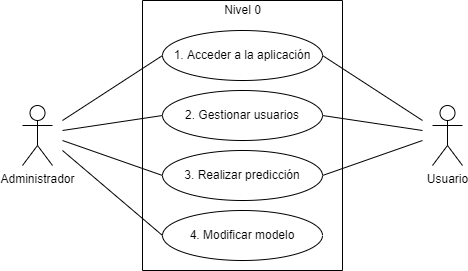
\includegraphics[width=1\textwidth]{nivel_0}
	\caption{Nivel 0 del diagrama de casos de uso.}
	\label{fig:nivel_0}
\end{figure}

\begin{figure}[h]
	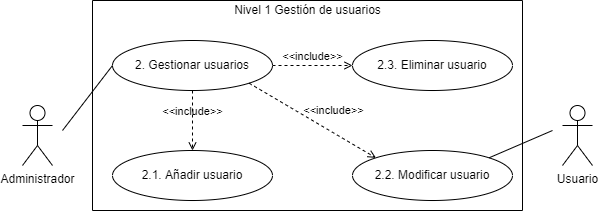
\includegraphics[width=1\textwidth]{gestion_usuarios}
	\caption{Nivel 1 Gestión de usuarios del diagrama de casos de uso.}
	\label{fig:gestion_usuarios}
\end{figure}

\subsection{Especificación de los casos de uso}
Las redacciones de los casos de uso de los diagramas anteriores, tablas \ref{tab:cu1}, \ref{tab:cu2}, \ref{tab:cu2_1}, \ref{tab:cu2_2}, \ref{tab:cu2_3}, \ref{tab:cu3} y \ref{tab:cu4} son las siguientes:

\begin{table}
	\begin{center}
		\begin{tabular}{| c | c | c |}
			\noalign{\hrule height 1.25pt}
			\rowcolor{gray!50}
			\multicolumn{3}{!{\vrule width 1.25pt} p{13.75cm} !{\vrule width 1.25pt}}{CU-1 Acceder a la aplicación} \\ \noalign{\hrule height 1.25pt}
			Dependencias & \multicolumn{2}{p{10cm} |}{
				\begin{itemize}
					\item RF-1 Restricción de acceso a la aplicación.
					\item RF-1.1 Acceso.
					\item RF-1.2 Administración.
				\end{itemize}} \\ \hline
			Actores & \multicolumn{2}{p{10cm} |}{Administrador y usuario} \\ \hline
			Precondición & \multicolumn{2}{p{10cm} |}{No hay ninguna sesión iniciada.} \\ \hline
			Descripción & \multicolumn{2}{p{10cm} |}{Se accede a la aplicación utilizando un nombre de usuario y una contraseña.} \\ \hline
			Secuencia normal & Paso & Acción \\ \cline{2-3}
			& 1 & \multicolumn{1}{p{8.75cm} |}{Se escribe el nombre de usuario y la contraseña para acceder.} \\ \cline{2-3}
			& 2 & \multicolumn{1}{p{8.75cm} |}{El servidor comprueba si es correcto y permite acceder al usuario.} \\ \hline
			Postcondición & \multicolumn{2}{p{10cm} |}{El usuario accede a la aplicación.} \\ \hline
			Excepciones & Paso & Acción \\ \cline{2-3}
			& 2 & \multicolumn{1}{p{8.75cm} |}{Si el nombre de usuario y/o la contraseña no son correctos no se accederá a la aplicación y se mostrará un error.} \\ \hline
			Comentarios & \multicolumn{2}{p{10cm} |}{Si el usuario no ha iniciado sesión sólo podrá acceder a esta ventana.} \\ \hline
		\end{tabular}
			\caption{Caso de uso 1: Acceder a la aplicación.}
			\label{tab:cu1}
	\end{center}
\end{table}

\begin{table}
	\begin{center}
		\begin{tabular}{| c | c | c |}
			\noalign{\hrule height 1.25pt}
			\rowcolor{gray!50}
			\multicolumn{3}{!{\vrule width 1.25pt} p{13.75cm} !{\vrule width 1.25pt}}{CU-2 Gestionar usuarios} \\ \noalign{\hrule height 1.25pt}
			Dependencias & \multicolumn{2}{p{10cm} |}{
				\begin{itemize}
					\item RF-2 Gestión de usuarios.
			\end{itemize}} \\ \hline
			Actores & \multicolumn{2}{p{10cm} |}{Administrador} \\ \hline
			Precondición & \multicolumn{2}{p{10cm} |}{Haber iniciado sesión con el usuario administrador.} \\ \hline
			Descripción & \multicolumn{2}{p{10cm} |}{Se muestran los usuarios registrados y las operaciones de añadir, modificar y eliminar.} \\ \hline
			Secuencia normal & Paso & Acción \\ \cline{2-3}
			& 1 & \multicolumn{1}{p{8.75cm} |}{Se accede a la ventana de gestión de usuarios.} \\ \hline
			Postcondición & \multicolumn{2}{p{10cm} |}{Se puede realizar la gestión de usuarios.} \\ \hline
			Excepciones & Paso & Acción \\ \cline{2-3}
			& 1 & \multicolumn{1}{p{8.75cm} |}{Si no se inicia sesión, el servidor redirigirá el acceso a la ventana de inicio de sesión.} \\ \hline
			& 1 & \multicolumn{1}{p{8.75cm} |}{Si el usuario no es el administrador, el servidor redirigirá el acceso a la ventana inicial.}  \\ \hline
		\end{tabular}
		\caption{Caso de uso 2: Gestionar usuarios.}
		\label{tab:cu2}
	\end{center}
\end{table}

\begin{table}
	\begin{center}
		\begin{tabular}{| c | c | c |}
			\noalign{\hrule height 1.25pt}
			\rowcolor{gray!50}
			\multicolumn{3}{!{\vrule width 1.25pt} p{13.75cm} !{\vrule width 1.25pt}}{CU-2.1 Añadir usuario} \\ \noalign{\hrule height 1.25pt}
			Dependencias & \multicolumn{2}{p{10cm} |}{
				\begin{itemize}
					\item RF-2.1 Añadir usuario.
			\end{itemize}} \\ \hline
			Actores & \multicolumn{2}{p{10cm} |}{Administrador} \\ \hline
			Precondición & \multicolumn{2}{p{10cm} |}{Haber iniciado sesión con el usuario administrador.} \\ \hline
			Descripción & \multicolumn{2}{p{10cm} |}{Se registra un nuevo usuario a la aplicación.} \\ \hline
			Secuencia normal & Paso & Acción \\ \cline{2-3}
			& 1 & \multicolumn{1}{p{8.75cm} |}{Se accede a la ventana de añadir usuario.} \\ \cline{2-3}
			& 2 & \multicolumn{1}{p{8.75cm} |}{Se rellenan los campos del nuevo usuario: nombre completo, nombre de usuario y contraseña.} \\ \cline{2-3}
			& 3 & \multicolumn{1}{p{8.75cm} |}{Se almacenan los datos.}\\ \hline
			Postcondición & \multicolumn{2}{p{10cm} |}{Se añade un nuevo usuario.} \\ \hline
			Excepciones & Paso & Acción \\ \cline{2-3}
			& 1 & \multicolumn{1}{p{8.75cm} |}{Si no se inicia sesión, el servidor redirigirá el acceso a la ventana de inicio de sesión.} \\ \hline
			& 1 & \multicolumn{1}{p{8.75cm} |}{Si el usuario no es el administrador, el servidor redirigirá el acceso a la ventana inicial.} \\ \cline{2-3}
			& 2 & \multicolumn{1}{p{8.75cm} |}{Si no se han rellenado todos los campos no se podrá añadir el usuario.} \\ \cline{2-3}
			& 2 & \multicolumn{1}{p{8.75cm} |}{Si el usuario existe no se podrá añadir el usuario.} \\ \hline
		\end{tabular}
		\caption{Caso de uso 2.1: Añadir usuario.}
		\label{tab:cu2_1}
	\end{center}
\end{table}

\begin{table}
	\begin{center}
		\begin{tabular}{| c | c | c |}
			\noalign{\hrule height 1.25pt}
			\rowcolor{gray!50}
			\multicolumn{3}{!{\vrule width 1.25pt} p{13.75cm} !{\vrule width 1.25pt}}{CU-2.2 Modificar usuario} \\ \noalign{\hrule height 1.25pt}
			Dependencias & \multicolumn{2}{p{10cm} |}{
				\begin{itemize}
					\item RF-2.2 Modificar usuario.
			\end{itemize}} \\ \hline
			Actores & \multicolumn{2}{p{10cm} |}{Administrador} \\ \hline
			Precondición & \multicolumn{2}{p{10cm} |}{Haber iniciado sesión con el usuario administrador.} \\ \hline
			Descripción & \multicolumn{2}{p{10cm} |}{Se modifica un usuario existente de la aplicación.} \\ \hline
			Secuencia normal & Paso & Acción \\ \cline{2-3}
			& 1 & \multicolumn{1}{p{8.75cm} |}{Se accede a la ventana de modificar usuario.} \\ \cline{2-3}
			& 2 & \multicolumn{1}{p{8.75cm} |}{Se modifican los campos del usuario: nombre completo, nombre de usuario y contraseña.} \\ \cline{2-3}
			& 3 & \multicolumn{1}{p{8.75cm} |}{Se almacenan los datos.}\\ \hline
			Postcondición & \multicolumn{2}{p{10cm} |}{Se modifica el usuario existente.} \\ \hline
			& 1 & \multicolumn{1}{p{8.75cm} |}{Si no se inicia sesión, el servidor redirigirá el acceso a la ventana de inicio de sesión.} \\ \hline
			Excepciones & Paso & Acción \\ \cline{2-3}
			& 1 & \multicolumn{1}{p{8.75cm} |}{Si el usuario no es el administrador, el servidor redirigirá el acceso a la ventana inicial.} \\ \cline{2-3}
			& 2 & \multicolumn{1}{p{8.75cm} |}{Si no se han rellenado todos los campos no se podrá modificar el usuario.} \\ \cline{2-3}
			& 2 & \multicolumn{1}{p{8.75cm} |}{Si el usuario existe no se podrá modificar el usuario.} \\ \hline
		\end{tabular}
		\caption{Caso de uso 2.2: Modificar usuario.}
		\label{tab:cu2_2}
	\end{center}
\end{table}

\begin{table}
	\begin{center}
		\begin{tabular}{| c | c | c |}
			\noalign{\hrule height 1.25pt}
			\rowcolor{gray!50}
			\multicolumn{3}{!{\vrule width 1.25pt} p{13.75cm} !{\vrule width 1.25pt}}{CU-2.3 Eliminar usuario} \\ \noalign{\hrule height 1.25pt}
			Dependencias & \multicolumn{2}{p{10cm} |}{
				\begin{itemize}
					\item RF-2.3 Eliminar usuario.
			\end{itemize}} \\ \hline
			Actores & \multicolumn{2}{p{10cm} |}{Administrador} \\ \hline
			Precondición & \multicolumn{2}{p{10cm} |}{Haber iniciado sesión con el usuario administrador.} \\ \hline
			Descripción & \multicolumn{2}{p{10cm} |}{Se elimina un usuario existente de la aplicación.} \\ \hline
			Secuencia normal & Paso & Acción \\ \cline{2-3}
			& 1 & \multicolumn{1}{p{8.75cm} |}{Se selecciona el usuario que se desea eliminar} \\ \cline{2-3}
			& 2 & \multicolumn{1}{p{8.75cm} |}{Se confirma el usuario que se desea eliminar.} \\ \hline
			Postcondición & \multicolumn{2}{p{10cm} |}{Se elimina el usuario.} \\ \hline
			Excepciones & Paso & Acción \\ \cline{2-3}
			& 1 & \multicolumn{1}{p{8.75cm} |}{Si no se inicia sesión, el servidor redirigirá el acceso a la ventana de inicio de sesión.} \\ \hline
			& 1 & \multicolumn{1}{p{8.75cm} |}{Si el usuario no es el administrador, el servidor redirigirá el acceso a la ventana inicial.} \\ \hline
		\end{tabular}
		\caption{Caso de uso 2.3: Eliminar usuario.}
		\label{tab:cu2_3}
	\end{center}
\end{table}

\begin{table}
	\begin{center}
		\begin{tabular}{| c | c | c |}
			\noalign{\hrule height 1.25pt}
			\rowcolor{gray!50}
			\multicolumn{3}{!{\vrule width 1.25pt} p{13.75cm} !{\vrule width 1.25pt}}{CU-3 Realizar predicción} \\ \noalign{\hrule height 1.25pt}
			Dependencias & \multicolumn{2}{p{10cm} |}{
				\begin{itemize}
					\item RF-3 Subida de datos al servidor.
					\item RF-3.1 Subida de vídeos.
					\item RF-3.2 Introducción de datos.
					\item RF-4 Visualización del resultado.
			\end{itemize}} \\ \hline
			Actores & \multicolumn{2}{p{10cm} |}{Administrador y usuario} \\ \hline
			Precondición & \multicolumn{2}{p{10cm} |}{Haber iniciado sesión.} \\ \hline
			Descripción & \multicolumn{2}{p{10cm} |}{Se suben los datos para realizar la predicción.} \\ \hline
			Secuencia normal & Paso & Acción \\ \cline{2-3}
			& 1 & \multicolumn{1}{p{8.75cm} |}{Se accede a la ventana.} \\ \cline{2-3}
			& 2 & \multicolumn{1}{p{8.75cm} |}{El usuario sube el vídeo y los datos al servidor.} \\ \cline{2-3} 
			& 3 & \multicolumn{1}{p{8.75cm} |}{Se muestra el resultado de la predicción.} \\ \hline
			Postcondición & \multicolumn{2}{p{10cm} |}{El usuario obtiene una predicción.} \\ \hline
			Excepciones & Paso & Acción \\ \cline{2-3}
			& 1 & \multicolumn{1}{p{8.75cm} |}{Si no se inicia sesión, el servidor redirigirá el acceso a la ventana de inicio de sesión.} \\ \hline
		\end{tabular}
		\caption{Caso de uso 3: Realizar predicción.}
		\label{tab:cu3}
	\end{center}
\end{table}

\begin{table}
	\begin{center}
		\begin{tabular}{| c | c | c |}
			\noalign{\hrule height 1.25pt}
			\rowcolor{gray!50}
			\multicolumn{3}{!{\vrule width 1.25pt} p{13.75cm} !{\vrule width 1.25pt}}{CU-4 Modificar modelo} \\ \noalign{\hrule height 1.25pt}
			Dependencias & \multicolumn{2}{p{10cm} |}{
				\begin{itemize}
					\item RF-5 Modificar modelo.
			\end{itemize}} \\ \hline
			Actores & \multicolumn{2}{p{10cm} |}{Administrador} \\ \hline
			Precondición & \multicolumn{2}{p{10cm} |}{Haber iniciado sesión con el usuario administrador.} \\ \hline
			Descripción & \multicolumn{2}{p{10cm} |}{Se modifica el modelo de predicción.} \\ \hline
			Secuencia normal & Paso & Acción \\ \cline{2-3}
			& 1 & \multicolumn{1}{p{8.75cm} |}{Se accede a la ventana.} \\ \cline{2-3}
			& 2 & \multicolumn{1}{p{8.75cm} |}{Se sube el nuevo modelo.} \\ \hline
			Postcondición & \multicolumn{2}{p{10cm} |}{Las predicciones se harán con el nuevo modelo.} \\ \hline
			Excepciones & Paso & Acción \\ \cline{2-3}
			& 1 & \multicolumn{1}{p{8.75cm} |}{Si no se inicia sesión, el servidor redirigirá el acceso a la ventana de inicio de sesión.} \\ \cline{2-3}
			& 1 & \multicolumn{1}{p{8.75cm} |}{Si el usuario no es el administrador, el servidor redirigirá el acceso a la ventana inicial.} \\ \hline
		\end{tabular}
		\caption{Caso de uso 4: Modificar modelo.}
		\label{tab:cu4}
	\end{center}
\end{table}

		\apendice{Especificación de diseño}

\section{Introducción}
En esta sección se detallan los aspectos más importantes de la aplicación: los datos utilizados, los procedimientos de la aplicación, la arquitectura de la aplicación y el diseño de las interfaces.

\section{Diseño de datos}

\section{Diseño procedimental}

\section{Diseño arquitectónico}

\section{Diseño de interfaces}
En este apartado, se muestran los diseños realizados de la aplicación web con la función de mostrar las funcionalidades que tendría la aplicación web, además de mostrar una interfaz con aspecto amigable.

\subsection{Vista de usuario}
Las pantallas del usuario son idénticas a las del administrador con la diferencia de que los usuarios no tendrán las opciones de ``Gestionar usuarios'' y ``Modificar modelo'', en su lugar tendrán la opción ``Modificar usuario''. Además, tendrán ventanas restringidas a las que únicamente el usuario administrador podrá acceder. Las ventanas disponibles para los usuarios sin privilegios son las correspondientes a las figuras \ref{fig:inicio_de_sesion}, \ref{fig:inicio}, \ref{fig:resultado} y \ref{fig:modificar_usuario}.

\subsection{Vista de administrador}
Se muestra el diseño de las interfaces para un usuario con privilegios.
\begin{figure}[h]
	\frame{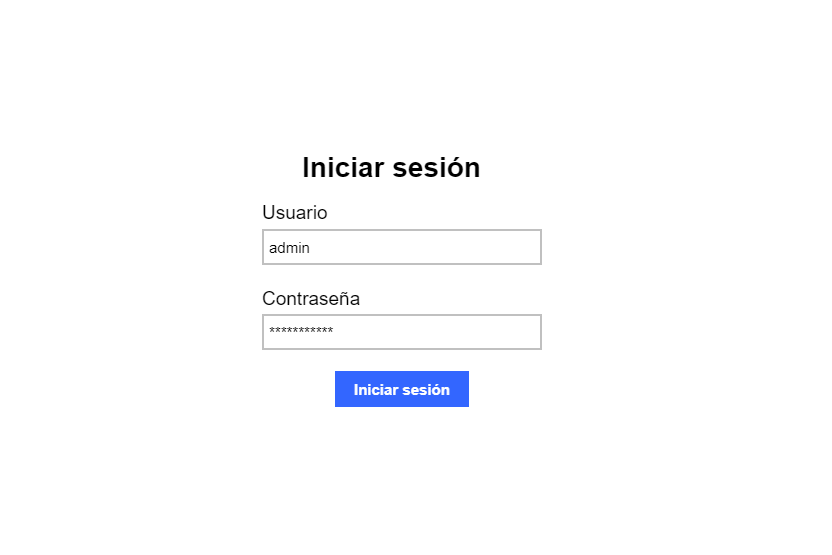
\includegraphics[width=1\textwidth]{inicio_de_sesion_admin}}
	\caption{Pantalla de inicio de sesión de un usuario administrador.}
	\label{fig:inicio_de_sesion}
\end{figure}

\begin{figure}[h]
	\frame{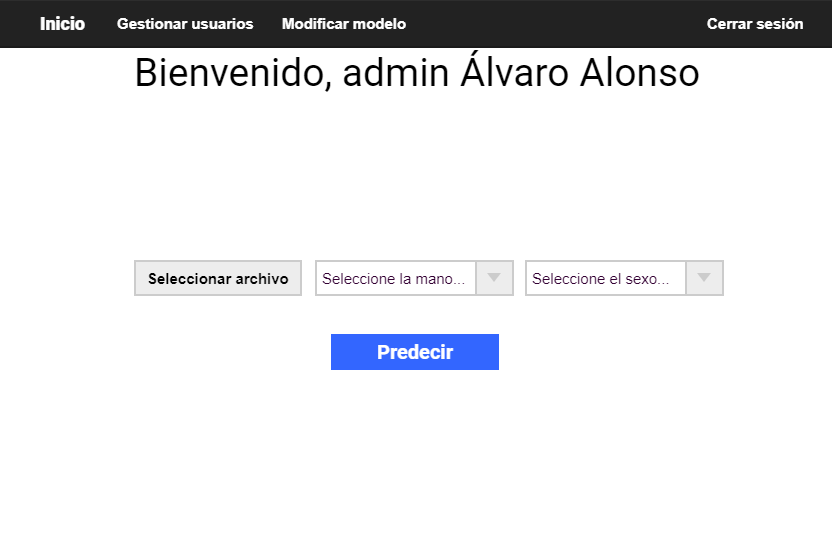
\includegraphics[width=1\textwidth]{inicio_admin}}
	\caption{Pantalla inicial de un usuario administrador.}
	\label{fig:inicio}
\end{figure}

\begin{figure}[h]
	\frame{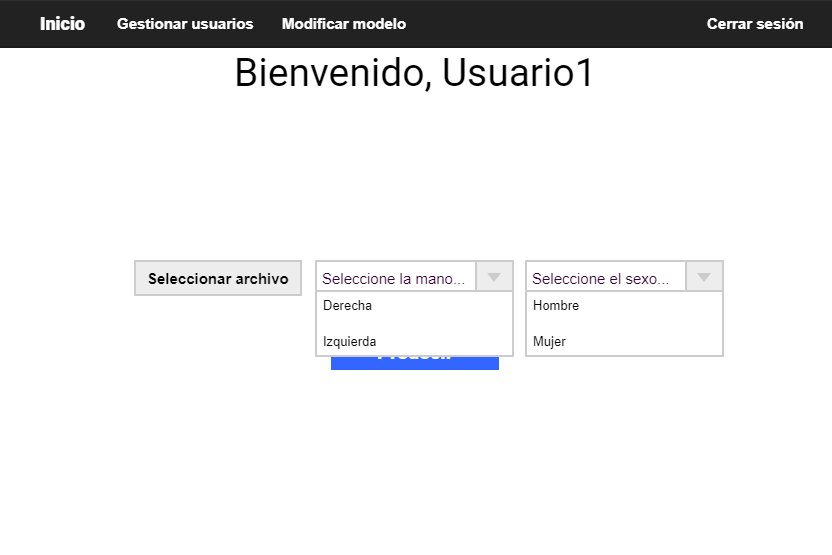
\includegraphics[width=1\textwidth]{inicio_admin_1}}
	\caption{Pantalla inicial de un usuario administrador con las listas desplegadas.}
	\label{fig:inicio_1}
\end{figure}

\begin{figure}[h]
	\frame{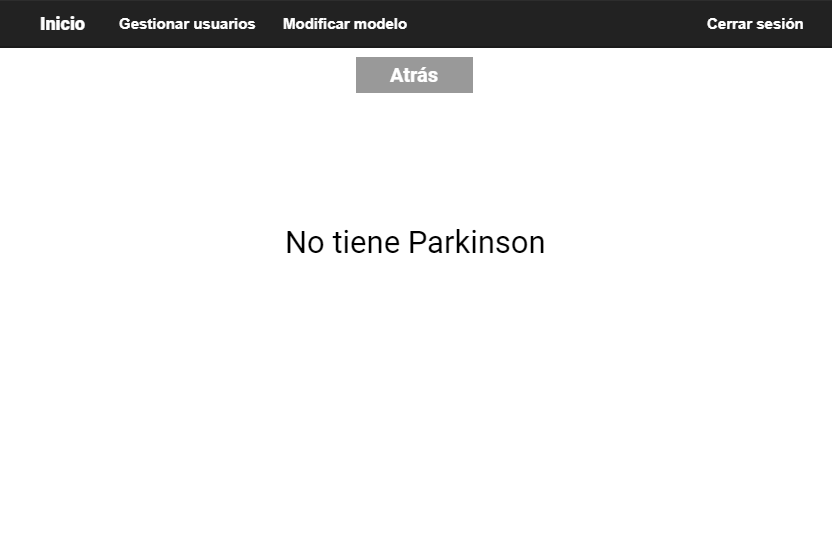
\includegraphics[width=1\textwidth]{resultado_admin}}
	\caption{Pantalla con el resultado de la predicción de un usuario administrador.}
	\label{fig:resultado}
\end{figure}

\begin{figure}[h]
	\frame{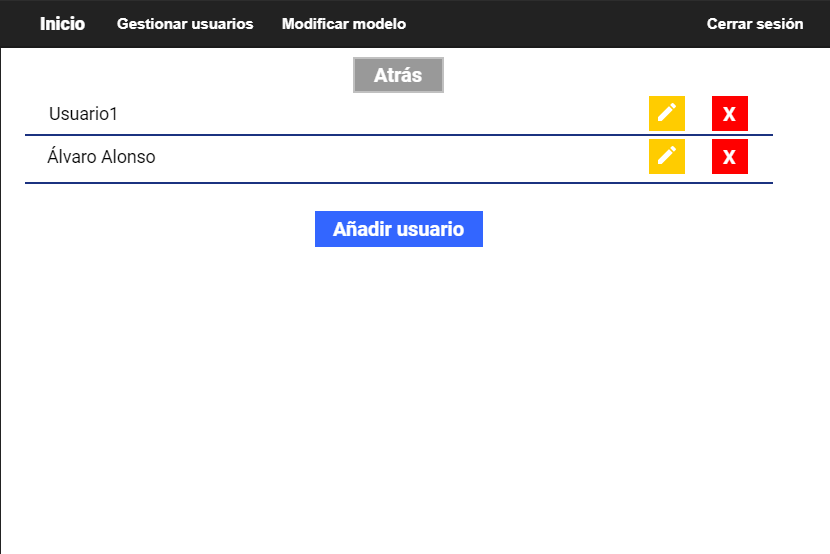
\includegraphics[width=1\textwidth]{gestionar_usuarios}}
	\caption{Pantalla con el listado de los usuarios dados de alta en la aplicación.}
	\label{fig:gestionar_usuarios}
\end{figure}

\begin{figure}[h]
	\frame{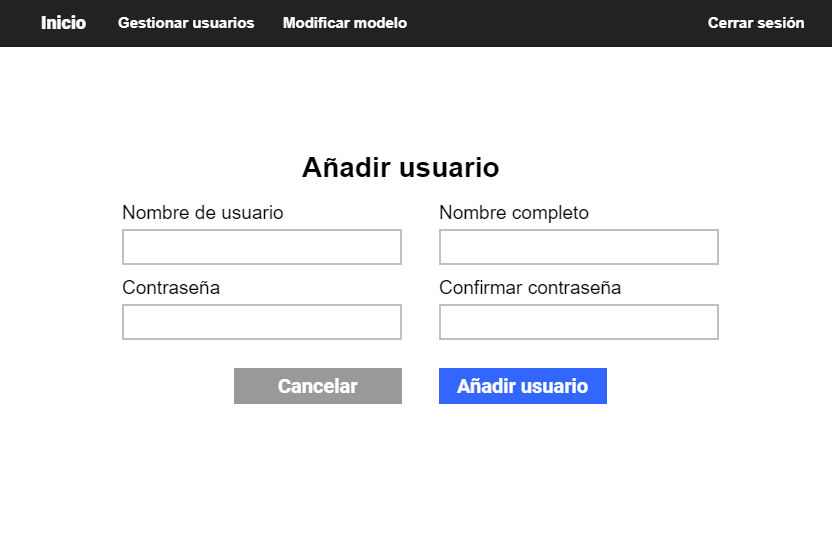
\includegraphics[width=1\textwidth]{agregar_usuario}}
	\caption{Pantalla con el formulario para dar de alta a un usuario.}
	\label{fig:agregar_usuario}
\end{figure}

\begin{figure}[h]
	\frame{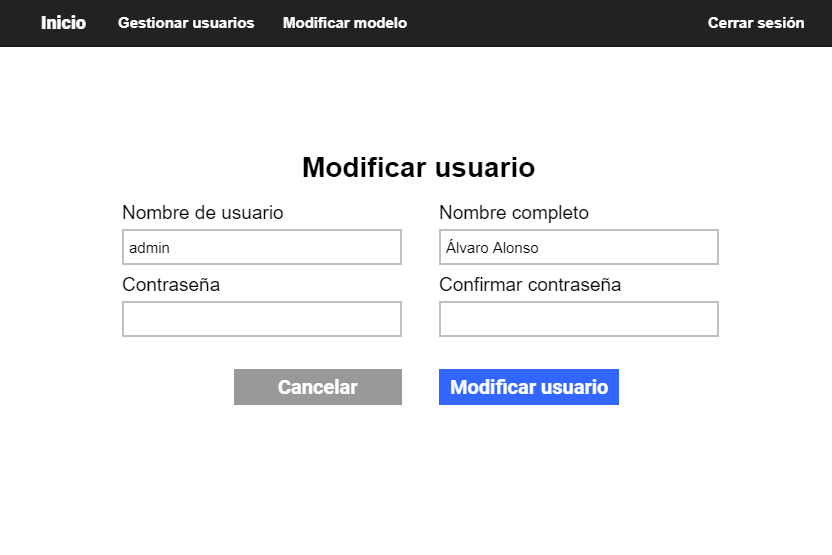
\includegraphics[width=1\textwidth]{modificar_usuario}}
	\caption{Pantalla con el formulario para modificar un usuario existente.}
	\label{fig:modificar_usuario}
\end{figure}

\begin{figure}[h]
	\frame{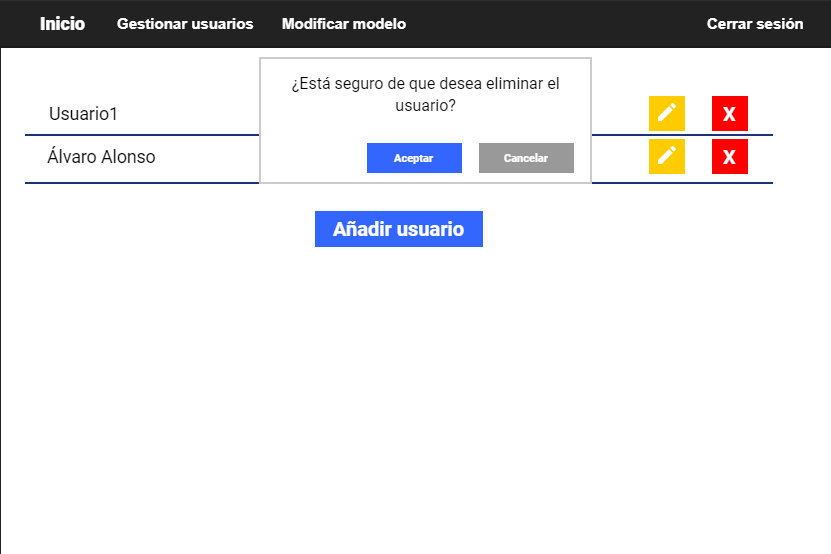
\includegraphics[width=1\textwidth]{eliminar_usuario}}
	\caption{Pantalla con la confirmación para borrar el usuario.}
	\label{fig:eliminar_usuario}
\end{figure}

\begin{figure}[h]
	\frame{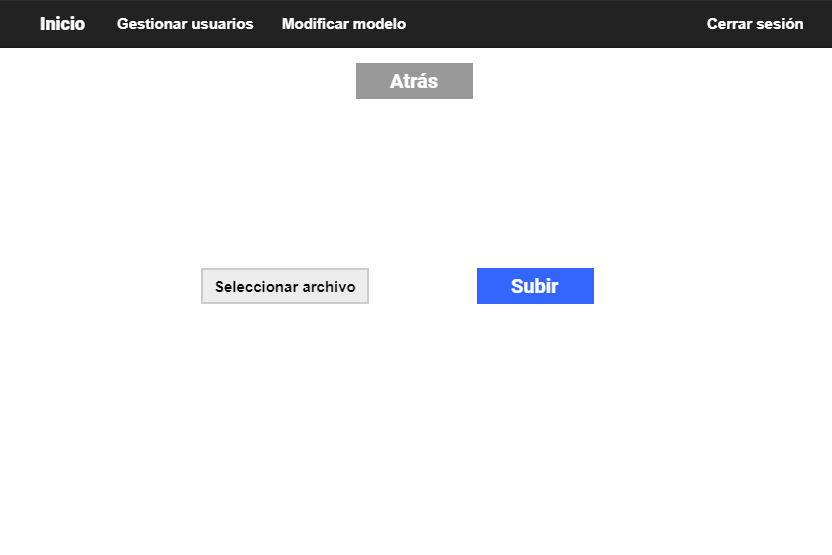
\includegraphics[width=1\textwidth]{modificar_modelo}}
	\caption{Pantalla con la subida del modelo al servidor.}
	\label{fig:modificar_modelo}
\end{figure}

		\apendice{Documentación técnica de programación}

\section{Introducción}
En este apartado, se detalla todo aquello que es necesario saber para comprender la aplicación web desde el punto de vista de un programador. También se detalla la estructura de directorios seguida para realización del proyecto.

\section{Estructura de directorios}
Los archivos realizados durante este proyecto se han subido al repositorio de GitHub, siguiendo una estructura. La estructura es la siguiente:

\begin{itemize}
	\item \textbf{/doc:} en esta carpeta se aloja toda la documentación del proyecto realizado. Esta carpeta además tiene otras en su interior y almacena los ficheros principales de la documentación, tanto en formato \LaTeX{} como en PDF, además de las bibliografías. Las carpetas interiores son:
		\begin{itemize}
			\item \textbf{/img:} en esta carpeta se alojan las imágenes de la documentación.
			\item \textbf{/tex:} en esta carpeta se alojan los ficheros de \LaTeX{} que conforman cada apartado de la memoria y los anexos.
		\end{itemize}
	\item \textbf{/notebooks:} en esta carpeta se alojan los archivos de Jupyter Notebook utilizados durante el desarrollo de este trabajo.
\end{itemize}

La estructura de ficheros seguida para el desarrollo de la aplicación es la siguiente:

\begin{itemize}
	\item \textbf{/impl:} esta carpeta contiene las clases de Python utilizadas en la aplicación para realizar diferentes funciones.
	\item \textbf{/modelo:} en esta carpeta se subirá el modelo para predecir. Únicamente habrá un archivo en esta carpeta, ya que al subir un nuevo modelo, el antiguo se eliminará.
	\item \textbf{/static:} esta carpeta contiene los archivos estáticos de la aplicación. Dentro hay otras tres carpetas, alojando cada una un tipo de archivo diferente:
	\begin{itemize}
		\item \textbf{/js:} esta carpeta contiene los archivos JavaScript utilizados en la aplicación web.
		\item \textbf{/img:} esta carpeta contiene las imágenes utilizadas en la aplicación web.
		\item \textbf{/css:} esta carpeta contiene los archivos CSS utilizados en la aplicación web.
	\end{itemize}
	\item \textbf{/templates:} esta carpeta contiene todos los archivos HTML de la aplicación. Alberga los archivos más generales y otras dos carpetas más, las cuales son:
	\begin{itemize}
		\item \textbf{/admin:} esta carpeta contiene todos los archivos HTML que tienen que ver con el usuario administrador, esto es, que sólo un usuario administrador puede ver renderizados.
		\item \textbf{/pred:} esta carpeta contiene todos los archivos HTML que tienen que ver con la predicción.
	\end{itemize}
	\item \textbf{/video:} esta carpeta contiene el vídeo que se va a procesar para realizar la predicción. Una vez termine la predicción, el vídeo se borrará del servidor.
\end{itemize}

\section{Manual del programador}

\section{Compilación, instalación y ejecución del proyecto}

\section{Pruebas del sistema}

		\apendice{Documentación de usuario}

\section{Introducción}
En esta sección, se explica al usuario qué necesita para poder utilizar la aplicación, cómo se instalaría y un manual de usuario para enseñarle cómo funciona.

\section{Requisitos de usuarios} \label{requisitos}
Los requisitos necesarios para poder utilizar la aplicación web son:

\begin{itemize}
	\item Tener un navegador que soporte HTML5, como Google Chrome o Microsoft Edge.
	\item Tener conexión a Internet.
\end{itemize}

Además, dado que es necesario estar dado de alta para utilizar la aplicación, se han preparado unos usuarios específicos para poder realizar pruebas en la aplicación desde un usuario con privilegios y otro sin privilegios:

\begin{itemize}
	\item \underline{Administrador:} 
	\begin{itemize}
		\item \textbf{Nombre de usuario:} admin.
		\item \textbf{Contraseña:} 1234.
	\end{itemize}
	\item \underline{Usuario:}
	\begin{itemize}
		\item \textbf{Nombre de usuario:} usuario.
		\item \textbf{Contraseña:} 1234.
	\end{itemize}
\end{itemize}

\section{Instalación}
Al tratarse de una aplicación web, no necesita nada más allá de un navegador web que soporte HTML5.

\section{Manual del usuario}
En esta sección se explica cómo utilizar la aplicación web.

\subsection{Inicio de sesión}
Nada más acceder a la aplicación web, aparecerá la pantalla de inicio de sesión que representa la figura \ref{fig:inicio_sesion_E}. Para acceder a ella, es necesario estar previamente dado de alta. Los usuarios indicados en el punto \ref{requisitos} pueden ser utilizados para acceder a la aplicación.

En caso de no escribir correctamente el usuario, aparecerá un mensaje indicando que el usuario es incorrecto, como se aprecia en la figura \ref{fig:usuario_no_encontrado_E}. Si la contraseña es incorrecta, aparecerá otro mensaje indicando que el error en el inicio de sesión ha sido la contraseña, tal y como se muestra en la figura \ref{fig:clave_incorrecta_E}, pero que el usuario es correcto.

Dependiendo de si se trata de un usuario con o sin privilegios, aparecerán unas opciones u otras.

\begin{figure}[ht]
	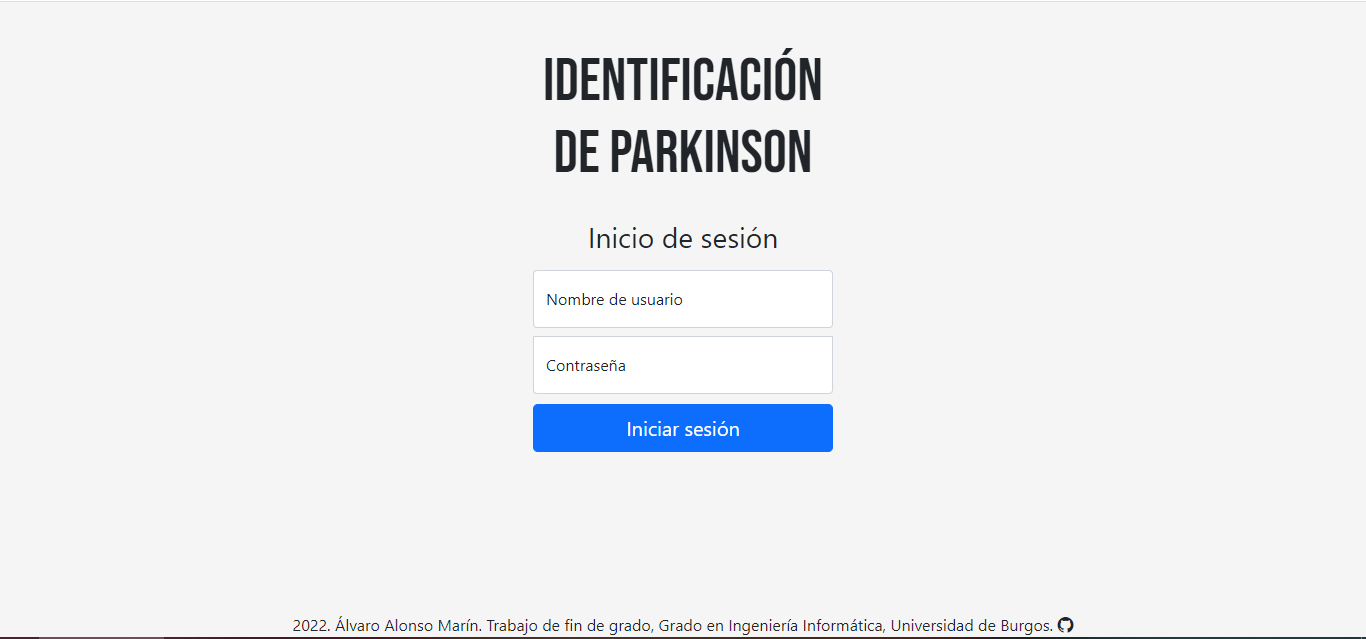
\includegraphics[width=1\textwidth]{inicio_sesion_E}
	\caption{Pantalla del inicio sesión de la aplicación web.}
	\label{fig:inicio_sesion_E}
\end{figure}

\begin{figure}[ht]
	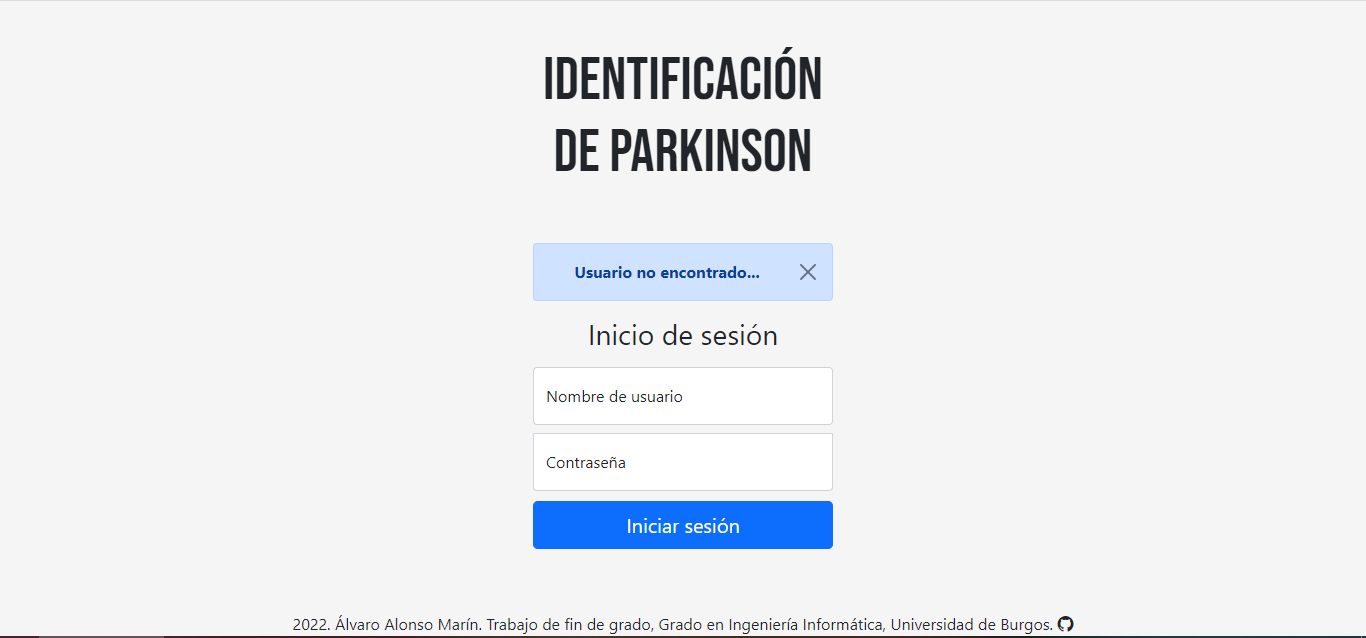
\includegraphics[width=1\textwidth]{usuario_no_encontrado}
	\caption{Pantalla del inicio sesión con el error de usuario no encontrado.}
	\label{fig:usuario_no_encontrado_E}
\end{figure}

\begin{figure}[ht]
	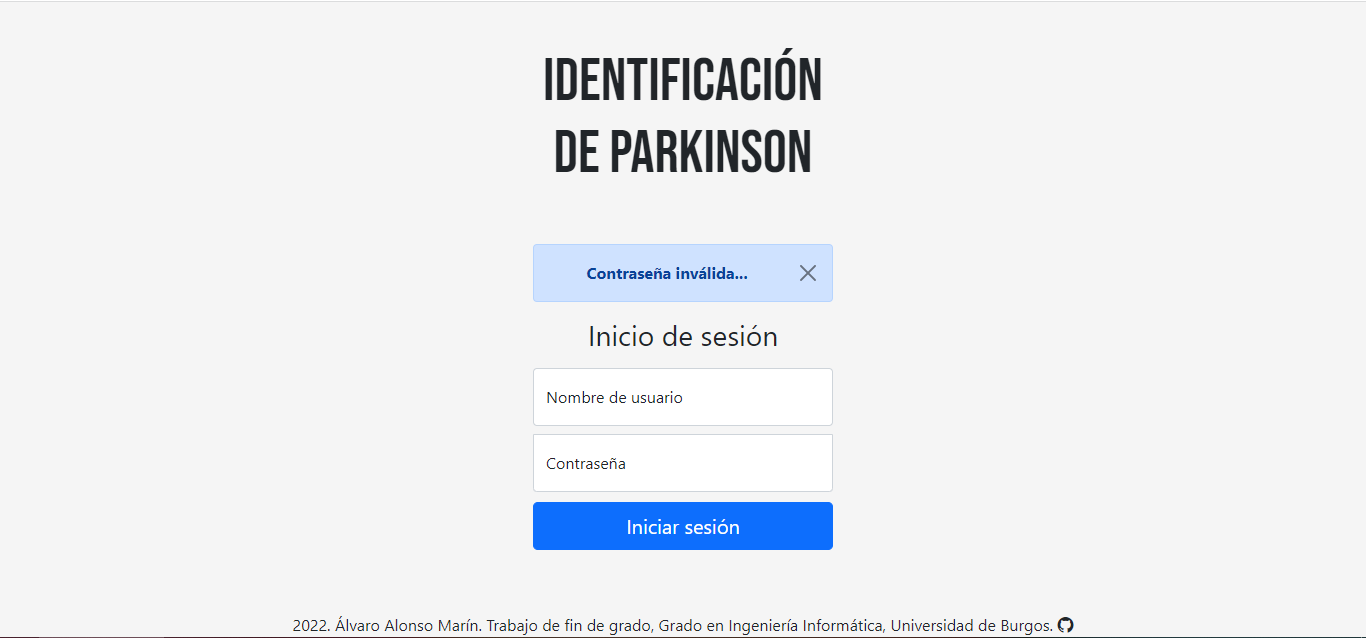
\includegraphics[width=1\textwidth]{clave_incorrecta}
	\caption{Pantalla del inicio sesión con el error de contraseña inválida.}
	\label{fig:clave_incorrecta_E}
\end{figure}

\subsection{Pantalla principal}

\subsubsection{Usuario administrador}
En caso de haber accedido con el usuario administrador, se podrán realizar más operaciones. En esta pantalla se podrá seleccionar el vídeo o arrastrarlo para realizar la predicción, además de seleccionar la mano y el sexo, tal y como se muestra en la figura \ref{fig:pantalla_principal_admin_E}.

\begin{figure}[ht]
	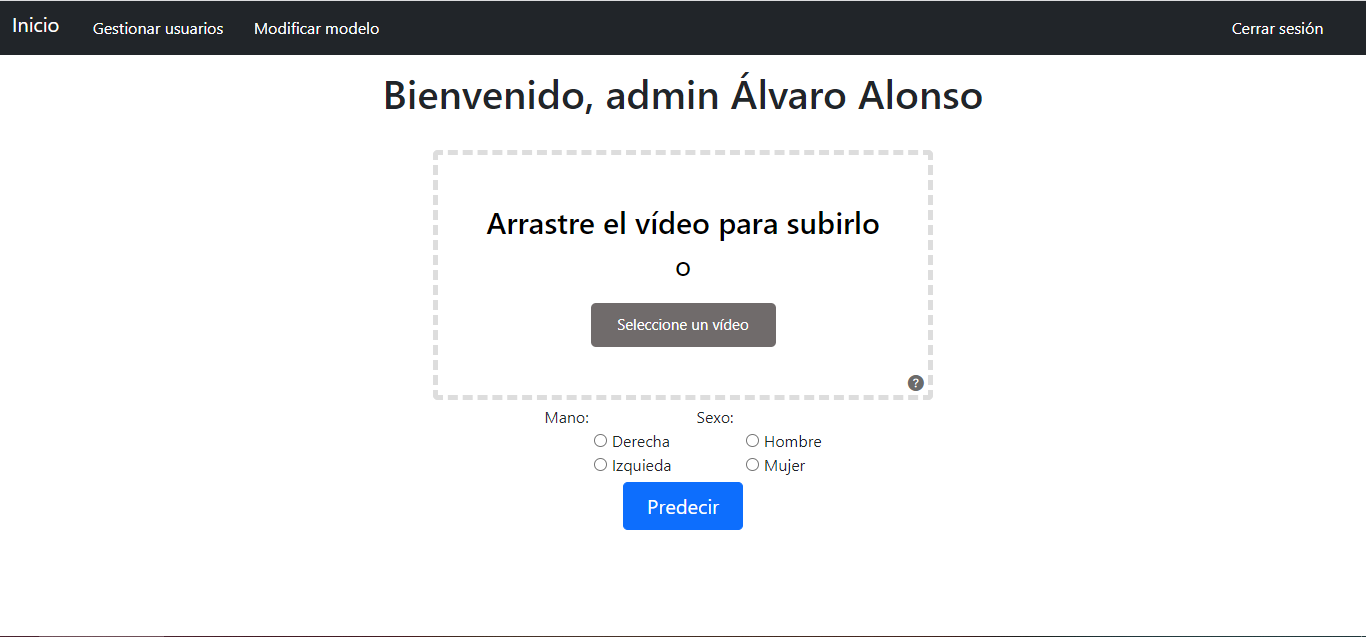
\includegraphics[width=1\textwidth]{pantalla_principal_admin_E}
	\caption{Pantalla principal del administrador para realizar la predicción.}
	\label{fig:pantalla_principal_admin_E}
\end{figure}

		
		
		\bibliographystyle{plain}
		\bibliography{bibliografiaAnexos}
		
	\end{document}